\documentclass[11pt,a4paper]{article}

% ---------- Sprache & Encoding ----------
\usepackage[utf8]{inputenc}
\usepackage[T1]{fontenc}
\usepackage{lmodern}

% ---------- Layout ----------
\usepackage[a4paper,margin=2.3cm]{geometry}
\usepackage{enumitem}
\usepackage{booktabs}
\usepackage{array}
\usepackage{tabularx}
\usepackage{graphicx}
\usepackage{amsmath,amssymb}
\usepackage{xcolor}
\usepackage{tcolorbox}
\tcbuselibrary{skins,breakable}
\usepackage{fancyhdr}
\usepackage[hidelinks]{hyperref}
\usepackage{titlesec}
\usepackage{needspace}

% ---------- Farben ----------
\definecolor{kfrblue}{HTML}{1F5C99}
\definecolor{warnorange}{HTML}{B45309}
\definecolor{warnbg}{HTML}{FFF3E0}
\definecolor{tipbg}{HTML}{EAF3EA}
\definecolor{tipgreen}{HTML}{2E7D32}

% ---------- Überschriften ----------
\titleformat{\section}{\large\bfseries\color{kfrblue}}{\thesection}{0.6em}{}
\titleformat{\subsection}{\normalsize\bfseries\color{kfrblue}}{\thesubsection}{0.6em}{}

% ---------- Kopf-/Fusszeile ----------
\pagestyle{fancy}
\fancyhf{}
\renewcommand{\headrulewidth}{0.4pt}
\fancyhead[L]{\small Physik 5.\,Klasse, Praktikum 08}
\fancyhead[R]{\small Theorieskript}
\fancyfoot[C]{\small\thepage}

% ---------- Boxen ----------
\newtcolorbox{achtungbox}[1][]{%
  colback=warnbg, colframe=warnorange, coltitle=white, colbacktitle=warnorange,
  boxrule=0.8pt, arc=2pt,
  left=6pt, right=6pt, top=4pt, bottom=4pt, breakable,
  title={\textbf{Achtung: darauf kommt es an}#1},
  fonttitle=\small, fontupper=\small
}
\newtcolorbox{tippbox}[1][]{%
  colback=tipbg, colframe=tipgreen, coltitle=white, colbacktitle=tipgreen,
  boxrule=0.8pt, arc=2pt,
  left=6pt, right=6pt, top=4pt, bottom=4pt, breakable,
  title={\textbf{Merke}#1},
  fonttitle=\small, fontupper=\small
}
\setlist[itemize]{leftmargin=1.4em, itemsep=2pt, topsep=3pt}
\setlist[enumerate]{leftmargin=1.6em, itemsep=2pt, topsep=3pt}

% ---------- einfache Einheiten-Makros (kein siunitx nötig) ----------
\newcommand{\SI}[2]{#1\,#2}
\newcommand{\milli}{m}
\newcommand{\meter}{m}

\begin{document}
\thispagestyle{empty}

% ---------- Titelblock ----------
\begin{center}
  {\color{kfrblue}\Large\bfseries Theorieskript: Linsenoptik}\\[2pt]
  {\normalsize Begleitmaterial zu Praktikum 08 (Linsenabbildung an der Sammellinse) \textbar\ Kantonsschule Freudenberg, Physik 5.\ Klasse}
\end{center}

\vspace{10pt}
\hrule
\vspace{10pt}

\noindent
Dieses Skript deckt die optischen Grundlagen ab, die für Praktikum~08 gebraucht werden: wie eine Sammellinse Bilder erzeugt, die drei Hauptstrahlen zur Konstruktion eines Bildpunkts, die Grössen Gegenstandsweite/-grösse und Bildweite/-grösse, sowie die Herleitung von Abbildungsgleichung und Abbildungsmassstab. Es kann vor dem Praktikum gelesen oder im Unterricht besprochen werden. Für die allgemeinen Regeln der Fehlerrechnung wird auf das Theorieskript zu Praktikum~01 verwiesen, hier wird in Abschnitt~7 nur die dort fehlende Kehrwertregel hergeleitet und auf beide Aussagen des Praktikums angewendet.

% ======================================================
\section{Von der Brechung zur Sammellinse}

Wie ihr in Praktikum~09 (Reflexion und Brechung) gemessen habt, wird Licht beim Übergang zwischen zwei Stoffen unterschiedlicher Brechzahl gemäss dem Brechungsgesetz von Snellius abgelenkt. Eine \textbf{\emph{Sammellinse}} (auch Konvexlinse) ist beidseitig gewölbt und nutzt genau diesen Effekt: An der gekrümmten Oberfläche wird jeder Lichtstrahl abhängig davon, wo er auf die Linse trifft, unterschiedlich stark gebrochen. Parallel zur optischen Achse einfallende Strahlen werden dadurch so gebrochen, dass sie sich alle in einem einzigen Punkt hinter der Linse schneiden, dem \textbf{\emph{Brennpunkt}}.

\begin{center}
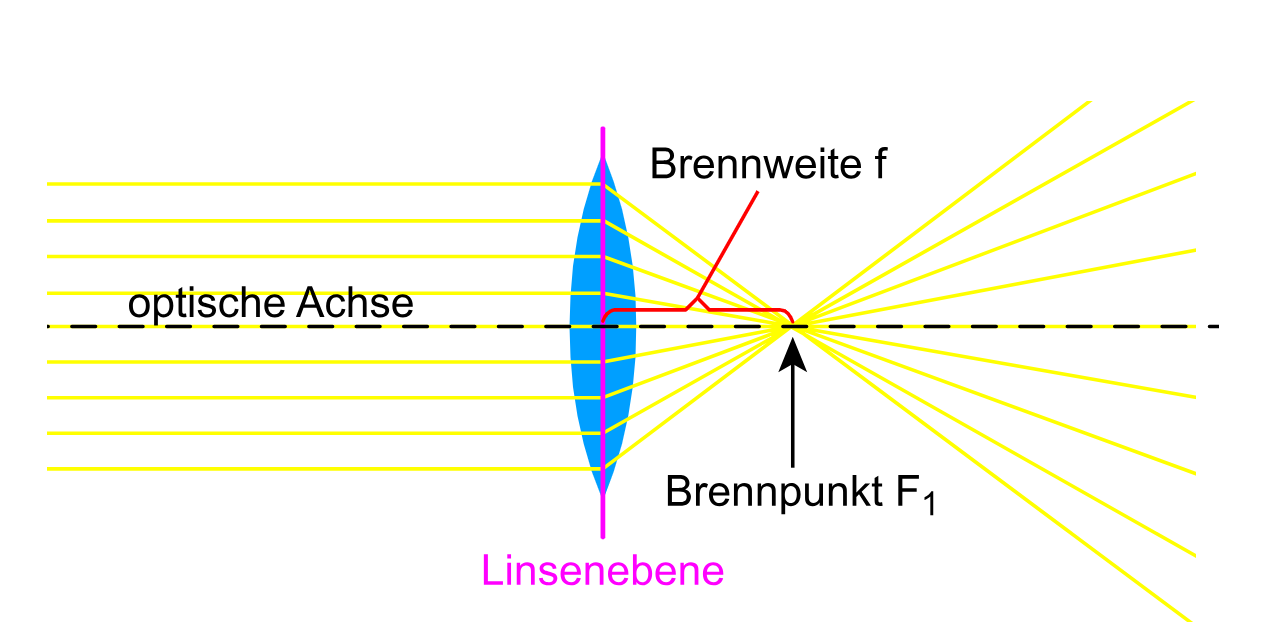
\includegraphics[width=0.72\linewidth]{Bilder/Brennweite.png}
\end{center}

Der Abstand zwischen der Linsenebene und dem Brennpunkt heisst \textbf{\emph{Brennweite}} $f$ (Einheit: $\mathrm{mm}$ oder $\mathrm{cm}$). Da eine Sammellinse Licht von beiden Seiten bündeln kann, besitzt sie zwei Brennpunkte, $F_1$ auf der Bildseite und $F_2$ auf der Gegenstandsseite, beide im gleichen Abstand $f$ von der Linsenebene. Je stärker eine Linse gekrümmt ist, desto stärker bricht sie das Licht und desto kleiner ist ihre Brennweite. Im Praktikum verwendet ihr eine Linse mit $f=\SI{75}{\milli\meter}$ (steht auf der Fassung: \emph{75\,mm FOCAL LENGTH}).

% ======================================================
\section{Bildkonstruktion: die drei Hauptstrahlen}

Um zu bestimmen, wo und wie eine Sammellinse das Bild eines Gegenstandspunkts $P$ erzeugt, genügt es, zwei beliebige von $P$ ausgehende Strahlen nach der Brechung zu verfolgen und ihren Schnittpunkt $P'$ zu suchen. In der Praxis wählt man dafür drei besonders einfach konstruierbare Strahlen, die \textbf{\emph{Hauptstrahlen}}:

\begin{itemize}
  \item \textbf{\emph{Parallelstrahl}}: verläuft von $P$ parallel zur optischen Achse zur Linse und wird danach durch den bildseitigen Brennpunkt $F_1$ gebrochen.
  \item \textbf{\emph{Brennpunktstrahl}}: verläuft von $P$ durch den gegenstandsseitigen Brennpunkt $F_2$ zur Linse und verlässt sie danach parallel zur optischen Achse.
  \item \textbf{\emph{Mittelpunktstrahl}}: verläuft von $P$ geradewegs durch den Mittelpunkt der Linse hindurch, ohne Richtungsänderung (die Linse ist in der Mitte näherungsweise wie eine planparallele Platte).
\end{itemize}

\begin{center}
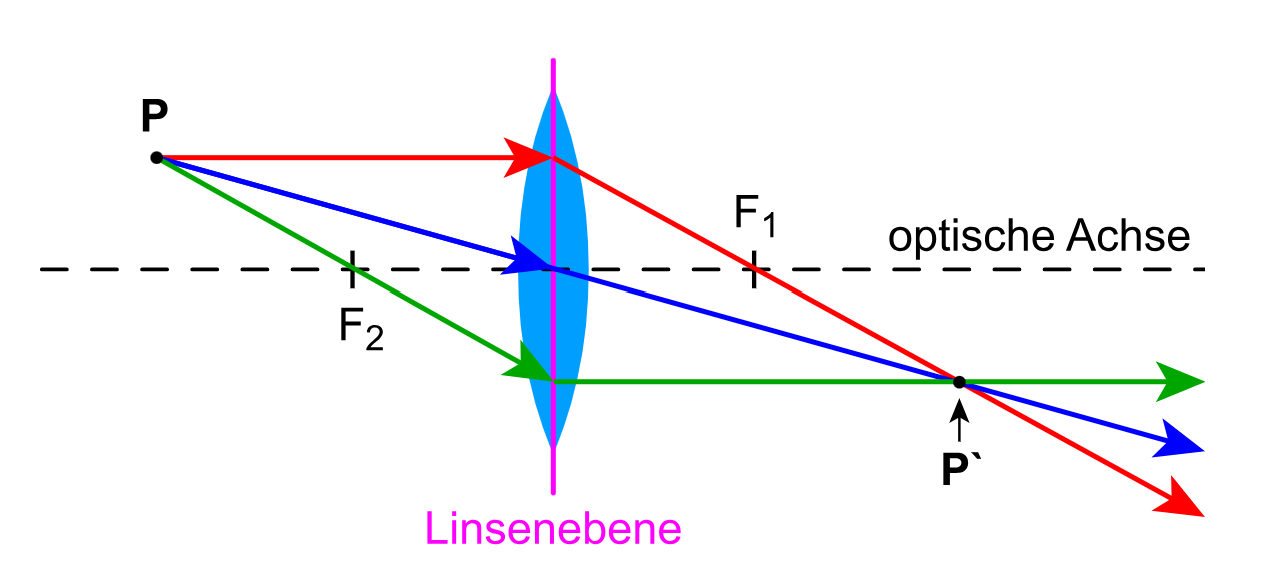
\includegraphics[width=0.85\linewidth]{Bilder/Abbildungspunkt.png}
\end{center}

Alle drei Strahlen (rot: Parallelstrahl, grün: Brennpunktstrahl, blau: Mittelpunktstrahl) schneiden sich nach der Linse im selben Punkt $P'$, dem Bildpunkt. Das ist kein Zufall, sondern eine Konsequenz des Brechungsgesetzes an der gekrümmten Linsenoberfläche; für die praktische Konstruktion genügen bereits zwei der drei Strahlen, der dritte dient zur Kontrolle.

% ======================================================
\section{Gegenstands- und Bildgrössen}

Um ein ausgedehntes Objekt (nicht nur einen einzelnen Punkt $P$) abzubilden, braucht es vier Grössen:

\begin{center}
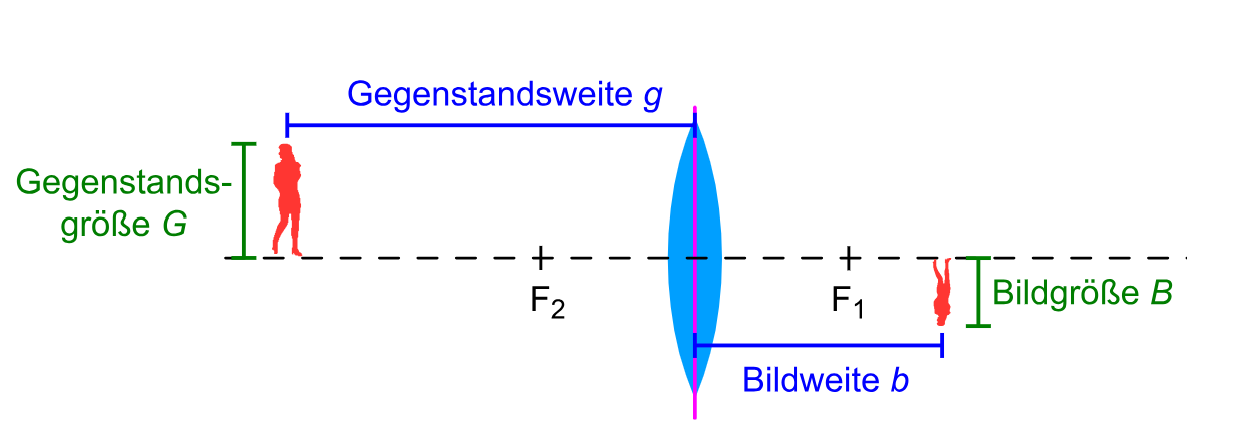
\includegraphics[width=0.82\linewidth]{Bilder/Gegenstand_Bild_weite.png}
\end{center}

\begin{itemize}
  \item \textbf{\emph{Gegenstandsweite}} $g$: Abstand zwischen Gegenstand und Linsenebene (Einheit: $\mathrm{mm}$).
  \item \textbf{\emph{Bildweite}} $b$: Abstand zwischen Linsenebene und Bild (Einheit: $\mathrm{mm}$).
  \item \textbf{\emph{Gegenstandsgrösse}} $G$: Höhe des Gegenstands senkrecht zur optischen Achse (Einheit: $\mathrm{mm}$).
  \item \textbf{\emph{Bildgrösse}} $B$: Höhe des Bilds senkrecht zur optischen Achse (Einheit: $\mathrm{mm}$).
\end{itemize}

In diesem Skript (und im Praktikum) werden alle vier Grössen als positive Längen behandelt, unabhängig davon, ob das Bild auf dem Kopf steht. Ob ein Bild aufrecht oder umgekehrt erscheint, wird separat in Worten angegeben, nicht über ein Vorzeichen von $B$.

% ======================================================
\section{Abbildungsmassstab}

\subsection{Herleitung über den Mittelpunktstrahl}

Der Mittelpunktstrahl verläuft unabgelenkt durch das Zentrum der Linse. Zusammen mit der optischen Achse bildet er auf der Gegenstandsseite ein rechtwinkliges Dreieck mit den Katheten $G$ und $g$, und auf der Bildseite ein rechtwinkliges Dreieck mit den Katheten $B$ und $b$. Beide Dreiecke liegen sich am Linsenmittelpunkt spiegelbildlich (scheitelrecht) gegenüber und sind deshalb \textbf{\emph{ähnlich}}: ihre Seitenverhältnisse stimmen überein.

\begin{center}
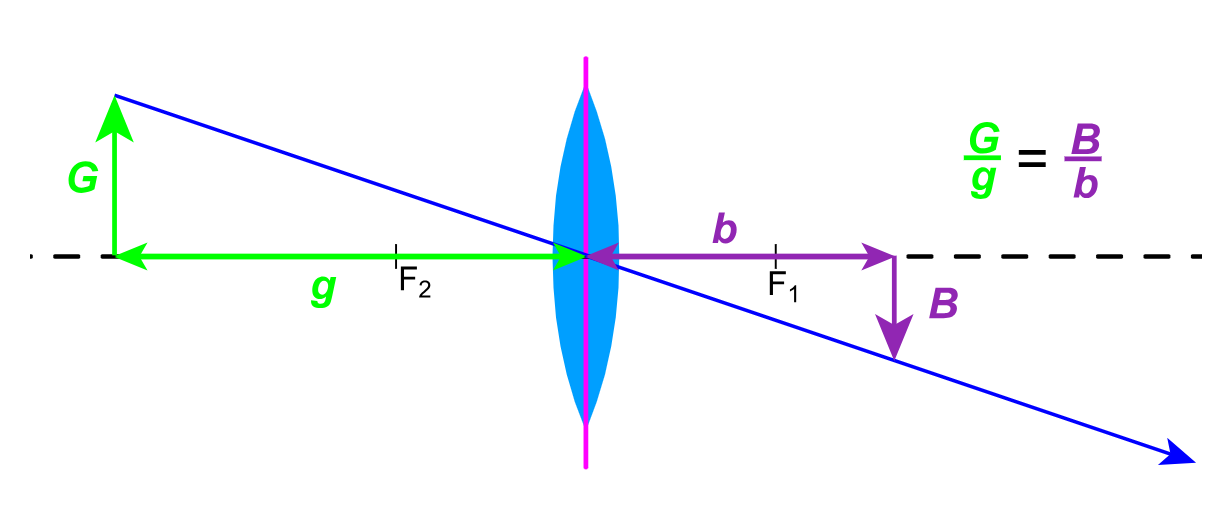
\includegraphics[width=0.75\linewidth]{Bilder/Linsengleichung_GBgb.png}
\end{center}

Aus der Ähnlichkeit der beiden Dreiecke folgt
\[
  \frac{G}{g} = \frac{B}{b}.
\]
Nach $B/G$ umgestellt (zuerst mit $g\cdot b$ durchmultiplizieren, danach durch $G\cdot g$ teilen):
\begin{align*}
  \frac{G}{g} &= \frac{B}{b} \\
  G\cdot b &= B\cdot g && \text{beide Seiten mit } g\cdot b \text{ multipliziert} \\
  \frac{b}{g} &= \frac{B}{G} && \text{beide Seiten durch } G\cdot g \text{ geteilt}
\end{align*}

\begin{tippbox}[: Abbildungsmassstab]
\[
  \boxed{\dfrac{B}{G} = \dfrac{b}{g}}
\]
Das Verhältnis von Bild- zu Gegenstandsgrösse ist gleich dem Verhältnis von Bild- zu Gegenstandsweite. Ist $b>g$, so ist das Bild grösser als der Gegenstand (Vergrösserung), ist $b<g$, ist es kleiner (Verkleinerung).
\end{tippbox}

% ======================================================
\section{Abbildungsgleichung}

\subsection{Herleitung über den Parallelstrahl}

Der Parallelstrahl verläuft von der Gegenstandsspitze (Höhe $G$) parallel zur Achse bis zur Linse und danach als Gerade durch $F_1$ zum Bildpunkt (Höhe $B$, Abstand $b$ von der Linse). Diese Gerade ist im Bild in Abschnitt~2 der rote Strahl von $P$ über die Linse und $F_1$ zu $P'$.

\begin{center}
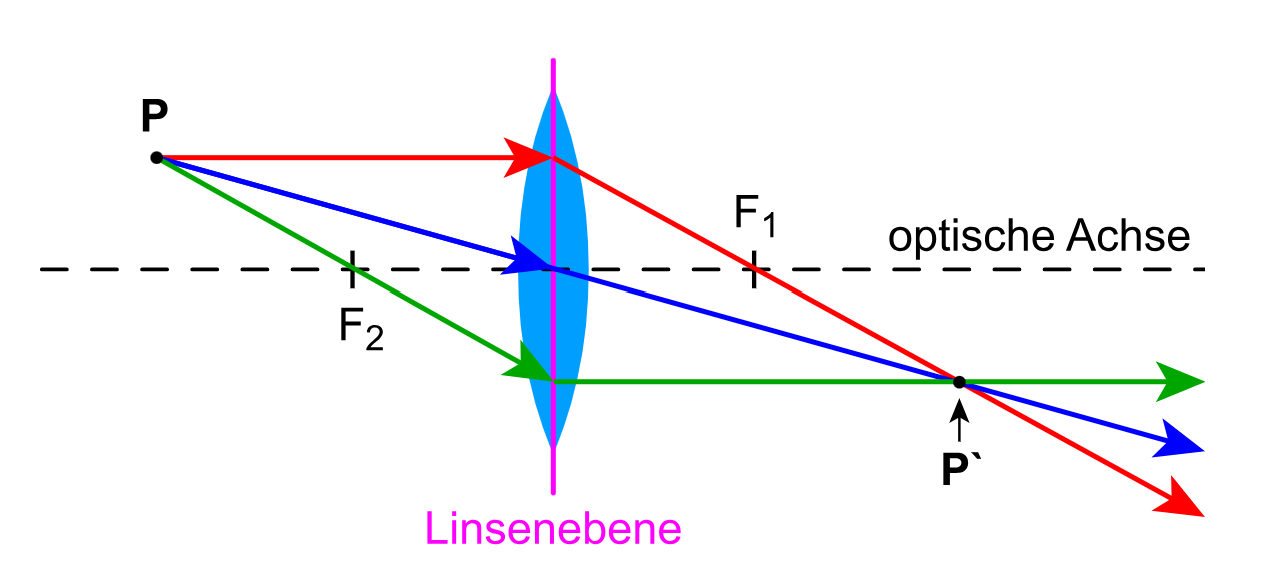
\includegraphics[width=0.85\linewidth]{Bilder/Abbildungspunkt.png}
\end{center}

Diese Gerade erzeugt zwei weitere ähnliche Dreiecke: eines zwischen Linse und $F_1$ (Kathete $f$ entlang der Achse, Kathete $G$ an der Linse), eines zwischen $F_1$ und dem Bild (Kathete $b-f$ entlang der Achse, Kathete $B$ am Bild). Auch diese beiden Dreiecke sind ähnlich (scheitelrechter Winkel bei $F_1$), also gilt
\[
  \frac{G}{f} = \frac{B}{b-f}.
\]

Mit der Beziehung $B = G\cdot\dfrac{b}{g}$ für den Abbildungsmassstab aus Abschnitt~4 lässt sich $B$ ersetzen:
\begin{align*}
  \frac{G}{f} &= \frac{G\cdot\frac{b}{g}}{b-f} && \text{$B$ eingesetzt} \\
  \frac{1}{f} &= \frac{\frac{b}{g}}{b-f} && \text{durch $G$ gekürzt} \\
  \frac{b-f}{f} &= \frac{b}{g} && \text{Kehrwert beider Seiten} \\
  \frac{b}{f} - 1 &= \frac{b}{g} && \text{Bruch aufgeteilt: } \tfrac{b-f}{f}=\tfrac{b}{f}-\tfrac{f}{f} \\
  \frac{b}{f} &= 1 + \frac{b}{g} && \text{$+1$ auf beiden Seiten} \\
  \frac{1}{f} &= \frac{1}{b} + \frac{1}{g} && \text{durch $b$ geteilt}
\end{align*}

\begin{tippbox}[: Abbildungsgleichung]
\[
  \boxed{\dfrac{1}{g} + \dfrac{1}{b} = \dfrac{1}{f}}
\]
Für jeden Gegenstandspunkt, der von derselben Linse scharf abgebildet wird, ergibt die Summe $\tfrac{1}{g}+\tfrac{1}{b}$ denselben Wert $\tfrac1f$, unabhängig davon, wie weit der Gegenstand von der Linse entfernt ist. Das ist die Beziehung, die ihr im Praktikum für mehrere $g$-Werte nachprüft.
\end{tippbox}

% ======================================================
\section{Spezialfälle: wie verändert sich das Bild mit $g$?}

Je nachdem, wie gross die Gegenstandsweite $g$ im Vergleich zur Brennweite $f$ ist, verändern sich Lage, Grösse und Art des Bilds deutlich. Die folgenden vier Fälle durchlauft ihr im Praktikum genau in dieser Reihenfolge, wenn ihr $g$ von $\SI{500}{\milli\meter}$ auf $\SI{50}{\milli\meter}$ verkleinert (bei $f=\SI{75}{\milli\meter}$):

\begin{center}
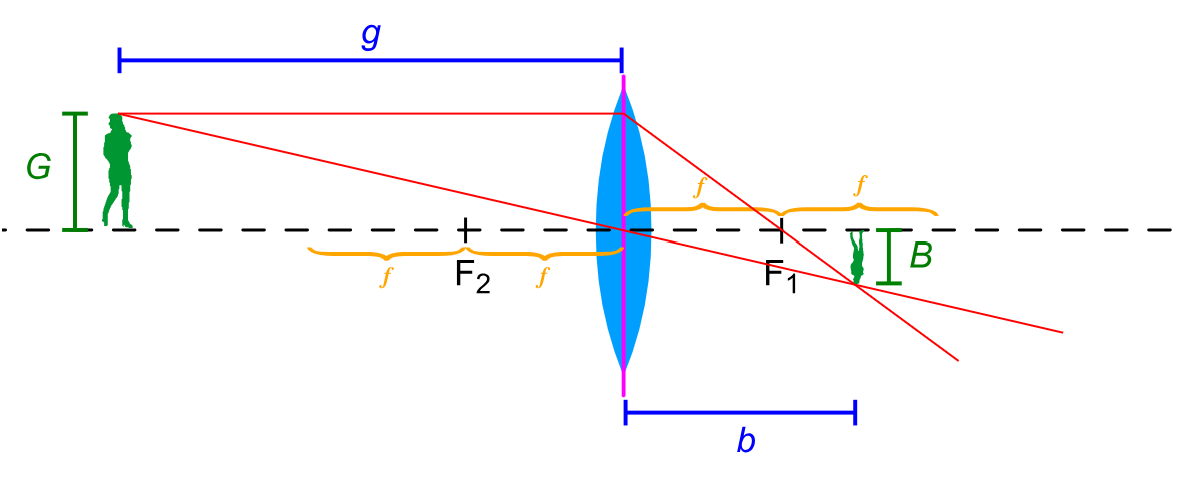
\includegraphics[width=0.8\linewidth]{Bilder/fall1.png}\\[2pt]
{\small \textbf{Fall 1:} $g>2f$: reelles, umgekehrtes, verkleinertes Bild ($f<b<2f$).}
\end{center}

\begin{center}
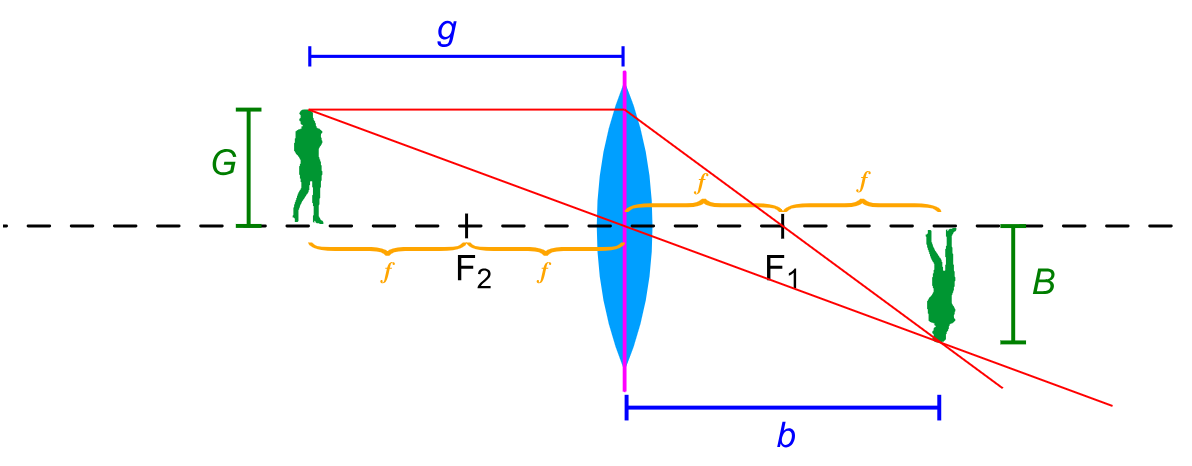
\includegraphics[width=0.8\linewidth]{Bilder/fall2.png}\\[2pt]
{\small \textbf{Fall 2:} $g=2f$: reelles, umgekehrtes, gleich grosses Bild ($b=2f$, $B=G$).}
\end{center}

\begin{center}
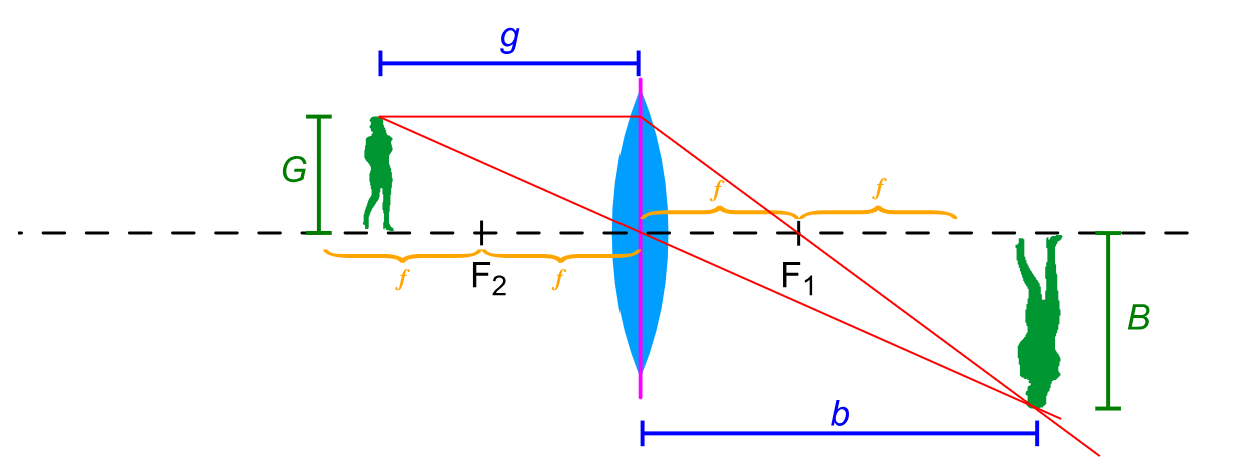
\includegraphics[width=0.8\linewidth]{Bilder/fall3.png}\\[2pt]
{\small \textbf{Fall 3:} $f<g<2f$: reelles, umgekehrtes, vergrössertes Bild ($b>2f$).}
\end{center}

\begin{center}
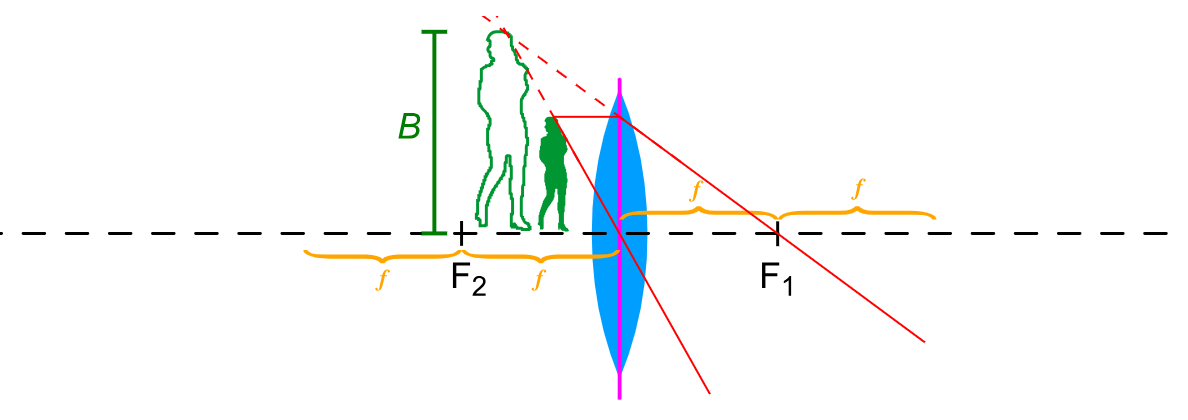
\includegraphics[width=0.8\linewidth]{Bilder/fall4.png}\\[2pt]
{\small \textbf{Fall 4:} $g<f$: \textbf{\emph{virtuelles}}, aufrechtes, vergrössertes Bild.}
\end{center}

In den ersten drei Fällen ist das Bild \textbf{\emph{reell}}: die gebrochenen Strahlen schneiden sich tatsächlich hinter der Linse und können dort auf einer Mattscheibe aufgefangen werden. Im vierten Fall ($g<f$) schneiden sich die gebrochenen Strahlen dagegen nicht mehr, nur ihre rückwärtigen Verlängerungen (gestrichelt) treffen sich vor der Linse. Ein solches \textbf{\emph{virtuelles}} Bild lässt sich nicht auf einer Mattscheibe auffangen, es ist nur sichtbar, wenn man selbst durch die Linse hindurchblickt, so wie bei einer Lupe.

\needspace{5cm}
\begin{achtungbox}
Beim Übergang zwischen Fall~3 und Fall~4, also bei $g=f$, liegt der Gegenstand genau im Brennpunkt $F_2$. Der Parallelstrahl und der Brennpunktstrahl verlassen die Linse dann beide parallel zur optischen Achse und schneiden sich nie, weder vor noch hinter der Linse. Es entsteht \textbf{\emph{kein}} Bild (weder reell noch virtuell): die gebrochenen Strahlen laufen für immer parallel weiter.
\end{achtungbox}

% ======================================================
\section{Fehlerfortpflanzung}

Im Praktikum werden alle vier Grössen $g$, $b$, $B$, $G$ von einer Skala abgelesen (Schienenmassstab bzw.\ Mattscheibenskala). Keine davon ist exakt bekannt. Für die Auswertung braucht ihr deshalb nicht nur die Messwerte selbst, sondern auch, wie sich deren Fehler auf $\tfrac1g+\tfrac1b$ und auf $\tfrac{B}{G}$ bzw.\ $\tfrac{b}{g}$ auswirken. Die allgemeinen Regeln der Fehlerrechnung (Additions-, Multiplikations- und Divisionsregel) sind im Theorieskript zu Praktikum~01 hergeleitet, Abschnitt~4.

\subsection{Kehrwertregel}

Für die Abbildungsgleichung braucht ihr den Fehler eines \textbf{\emph{Kehrwerts}} $z=1/x$ (für $x=g$ oder $x=b$), eine Regel, die im Skript zu Praktikum~01 nicht vorkommt. Ein Kehrwert $z=1/x$ ist ein Spezialfall der Division $z=a/x$ mit einem exakten Zähler $a=1$ (also $\Delta a=0$). Die Divisionsregel liefert für die relativen Fehler
\[
  \frac{\Delta z}{z} = \frac{\Delta a}{a} + \frac{\Delta x}{x} = 0 + \frac{\Delta x}{x} = \frac{\Delta x}{x}.
\]
Multipliziert man beide Seiten mit $z=1/x$, ergibt sich der absolute Fehler:
\[
  \Delta z = z\cdot\frac{\Delta x}{x} = \frac{1}{x}\cdot\frac{\Delta x}{x} = \frac{\Delta x}{x^2}.
\]

\begin{tippbox}[: Fehler des Kehrwerts]
\[
  \boxed{\Delta\!\left(\frac{1}{x}\right) = \frac{\Delta x}{x^2}}
\]
Je kleiner $x$ ist, desto stärker wirkt sich derselbe absolute Fehler $\Delta x$ auf $1/x$ aus (der Nenner $x^2$ wird kleiner). Diese Regel gilt für jede gemessene Grösse $x$, im Praktikum also sowohl für $g$ als auch für $b$.
\end{tippbox}

\subsection{Anwendung auf die Abbildungsgleichung}

Mit der Kehrwertregel für $x=g$ und $x=b$ und der Additionsregel für die Summe folgt
\[
  \boxed{\Delta\!\left(\frac1g+\frac1b\right) = \Delta\!\left(\frac1g\right)+\Delta\!\left(\frac1b\right) = \frac{\Delta g}{g^2}+\frac{\Delta b}{b^2}}.
\]
Beide Messunsicherheiten $\Delta g$ und $\Delta b$ tragen also zur Unsicherheit der Summe bei, nicht nur $\Delta b$.

\subsection{Anwendung auf den Abbildungsmassstab}

$B/G$ und $b/g$ sind beides Quotienten, die Divisionsregel liefert direkt
\[
  \boxed{\frac{\Delta(B/G)}{B/G} = \frac{\Delta B}{B}+\frac{\Delta G}{G}, \qquad \frac{\Delta(b/g)}{b/g} = \frac{\Delta b}{b}+\frac{\Delta g}{g}}.
\]
Für die Differenz $d=\tfrac bg-\tfrac BG$, die laut der Gleichung für den Abbildungsmassstab $0$ sein sollte, gilt nach der Additionsregel
\[
  \Delta d = \Delta\!\left(\frac bg\right)+\Delta\!\left(\frac BG\right).
\]

\begin{achtungbox}
$g$ und $b$ werden aus \emph{derselben} Schienenskala abgelesen (die Linsenposition kommt in beiden vor). Streng genommen sind ihre Fehler deshalb nicht ganz unabhängig voneinander. Für dieses Praktikum behandelt ihr $\Delta g$ und $\Delta b$ trotzdem als unabhängig. Das ist eine bewusste Vereinfachung, keine exakte Rechnung.
\end{achtungbox}

% ======================================================
\section{Zusammenfassung}
\begin{tippbox}[: alle Formeln auf einen Blick]
\begin{align*}
  \frac{1}{g} + \frac{1}{b} &= \frac{1}{f} &&\text{Abbildungsgleichung} \\
  \frac{B}{G} &= \frac{b}{g} &&\text{Abbildungsmassstab} \\
  \Delta\!\left(\frac{1}{x}\right) &= \frac{\Delta x}{x^2} &&\text{Fehlerfortpflanzung bei einem Kehrwert} \\
  \Delta\!\left(\frac1g+\frac1b\right) &= \frac{\Delta g}{g^2}+\frac{\Delta b}{b^2} &&\text{für die Abbildungsgleichung} \\
  \frac{\Delta(B/G)}{B/G} &= \frac{\Delta B}{B}+\frac{\Delta G}{G} &&\text{für den Abbildungsmassstab}
\end{align*}
\end{tippbox}

\end{document}
